\emph{The Times}  made the
same mistake when it published the scan of what the newspaper claimed
to be an internal US intelligence report on the paper's website in
2000~\cite{nyt-unediting-2003}. \emph{The Washington Post} made a
similar mistake in 2002 when it posted the demands of the DC
Sniper\cite{internet-forensics}.

This article shows
why PDF files have privacy risks that continue to befuddle their
users. It also explores the
metadata risks caused by the Office file format. Finally, it explores
some of the technical solutions that vendors have developed to address
these problems, as well as an obvious solution that 
word processors could adopt.

PDF files are not \emph{inherently dangerous}, perhaps, but they
demand respect. Security and Privacy professionals need to
understand why such leaks keep happening and how to stop them.

\section{Privacy Leaks in PDF}

PDF is based on PostScript, but instead of being designed as a general
purpose programming language that produce printed pages, PDF is a
specialized file format. Like PostScript, PDF has
commands for drawing lines, embedding fonts and displaying text. But PDF also has direct support for
document structure; a variety of image and video compression
algorithms; electronic forms; digital rights management; and
cryptography. PDF supports embedded JavaScript for form validation
and other kinds of automation. Any page in a PDF document can be
rendered without reference to any other. 

This rich support requires a complex reader that can interpret the
format, and such readers inevitably have flaws. Many of these flaws
have been exploited by attackers using cleverly constructed
PDF documents~\cite{5705599}. But whereas PDF exploits depend upon
implementation errors, PDF privacy leaks typically result from
properly formed files  containing information that is invisible but
readily extracted. To understand how privacy leaks take place, it
is important to understand how PDFs are created and a bit
about the PDF internal structure.

\subsection{Creating PDFs}

Users typically create PDF files in one of two ways. Users can
generate a PDF directly from an application program like word
processor or web browser.  Originally users would first ``print'' to a
PostScript (PS) file, then convert the PS to PDF using Adobe's
Acrobat Distiller. These days there are numerous drivers that allow
applications to ``print'' directly to a PDF file, and many application
programs can directly export to the format. PDF files created in this
manner contain actual fonts and characters that are rendered by the
output device. Such PDFs have sharp, crisp letters, text that can be
selected and copied, and files that are searchable. A happy side
effect is that these files tend to be relatively small, since the
internal data streams are compressed. These PDF files are 
\emph{accessible}, since people who are vision impaired can readily use
the documents by enlarging the text or using screen readers.

A second way to create PDF files is to scan a paper
document, producing a PDF file that is essentially a collection of
photographs. Even when scanned at 300 dots per inch, the
resulting documents can appear pixelated, mushy, and difficulty to read on a
computer screen, since the PDF reader is displaying a photograph of text,
rather than rendering text. The
text is not accessible---it cannot be selected, copied, searched, or
read with a screen reader. Such files also tend to be 10 to 100 times
larger than the PDF files created with the first
method. Unfortunately, many PDF files in circulation are scans because
the original paper documents were not prepared using a computer,
the original electronic files are no longer  available, or the
individuals that prepared the files did not have the tools or 
training to create an accessible PDF file.

Some PDF processing programs have the ability to process scanned text
with an optical character recognition (OCR) engine. Adobe's Acrobat
Pro's ``Recognize Text'' command will match  the picture in
the PDF file with letters or words that might have produced
it. Acrobat Pro can then modify the PDF file and place the recognized
text in a second layer underneath the scanned image. The result is a
scanned PDF  that is searchable but that preserves the
original image. Recognized text obscured by an image is an example of hidden text with
a genuinely useful purpose. Even if the recognition is slightly wrong, the
user sees the original picture, so the sense is preserved. Only text
search and extraction are impacted by OCR errors.

Acrobat 9 introduced a variant of OCR called
``ClearScan'' that creates a custom font for the each scanned
document based on the character bitmaps present in the document. The
program then replaces matching bitmaps on each page with characters
from the new font.  The result looks better, but when there is an OCR
error ClearScan can inadvertently produce apparent typos or even semantic changes in the resulting
document.

Surprisingly, the PDF standard itself does not make a distinction
between PDF files that are accessible and those that aren't. From the
point of view of the standard, a PDF is simply a file that contains
\emph{objects} (e.g.\ text drawing commands and fonts); a \emph{file
  structure} that describes how and where the objects are stored in
the file; a \emph{document structure} that describes how the objects
are used to create pages; and one or more \emph{content streams} that
describe how to display pages on the screen and how to print them.  The
power of  PDF comes from the ability to compose  these features in  many different ways. 


\subsection{Textual Privacy Leaks}

Many of the cases reported in the media in which private information
leaked out in PDF files appear to have resulted from the use of the
Microsoft Word ``Text Highlight'' tool (Figure~\ref{ms-tool}).  In
normal use, the tool is used to turn the background color of text from
white to yellow to attract
attention, similar to highlighting text with a
yellow marker. But Word does not use a translucent
color. Instead, the program prints highlighted text by first printing
the colored box, then the black text.

\begin{figure}
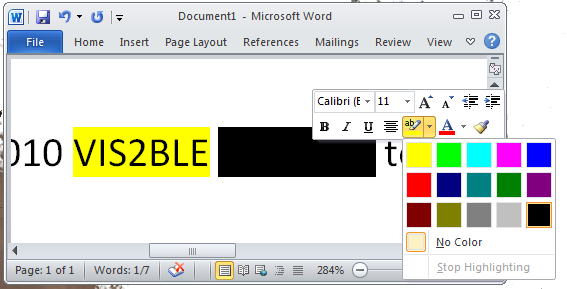
\includegraphics[width=3in]{ms-tool}
\caption{Microsoft Word 2010's highlight tool can be used to highlight
  text with different background colors. When the background is
  black, the text appears to be redacted, but it is still present.}\label{ms-tool}
\end{figure}

Privacy leaks can happen when
the user changes the highlight color from yellow to black. The result
is black text on a black box.  But Word still generates
instructions to print both the  box \emph{and} the 
text when printing to a PDF file (Figure~\ref{demo1}), and both can be
independently recovered. 

\begin{figure}
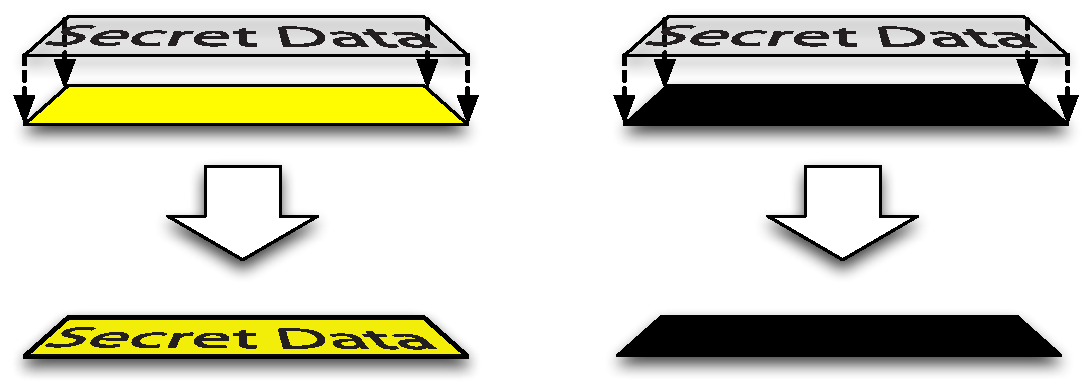
\includegraphics[width=\textwidth]{demo/fig2}
\caption{The Text Highlight tool places a colored box underneath the
  text. When the box is the same color of the text, the text appear to
  be absent, but it is still present.}\label{demo1}
\end{figure}

The behavior of Word is particularly pernicious because the resulting
text looks very similar to a document that has been redacted through
the official procedures used by many governments---obscuring sensitive
text with black boxes. Furthermore, there would likely be no
significant privacy leak if the document were printed and
distributed as hard copy---or if it were printed, scanned, and a non-accessible PDF
distributed. It is only the distribution of the PDF created directly
from the word processor that results in the leak.

The easiest way to recover the hidden text is with Acrobat Reader's
copy-and-paste commands:  copy the blacked out text and paste into
another document. Acrobat Reader's ``copy'' function places both plain text
and rich text on the computer's clipboard, but it doesn't copy the
text's background color. More dramatic demonstrations are possible
with PDF editing tools such as Adobe Illustrator or Inkscape. These tools understand the internal structure of PDF files
and allow objects on each page to be individually manipulated. With
Inkscape, for example, the box can be selected and then changed
from black to fuchsia (Figure~\ref{fuschia}), resulting in the highlighting of text that was intended to be
redacted. 

\begin{figure}
\includegraphics[width=\textwidth]{demo/fig1-before.png}\\
\includegraphics[width=\textwidth]{demo/fig1-after.png}
\caption{Black boxes created with the Text Highlight tool can be
  readily changed to a different color with PDF editing tools such as Inkscape.}\label{fuschia}
\end{figure}

The Text Highlight tool is not the only source of textual privacy
leaks. For example, in the case of the \emph{The
  Times}'s redaction error, the paper apparently scanned the report
into a PDF file, then
drew black boxes on the scanned pages using Adobe Photoshop 4.0 for
the Macintosh. Instead of drawing the black boxes directly on the
scanned bitmap, however, the boxes were placed in another Photoshop
layer---the application program's default behavior, so that
the files can be re-opened and the individual layers re-edited. Of course, this is not what
the editors at \emph{The Times}  intended. The problem could have
been averted if the Photoshop operator had simply ``flattened'' the
layers in the PDF file before it was made available on the newspaper's web server. 

\emph{The Washington Post} made a similar mistake on October 26, 2002,
when it published the scan of a four-page demand letter from the DC
Sniper on the paper's website. The sniper's letter included a demand
for \$10 million that the murderer wanted to be deposited in a debit
card account. \emph{The Post} attempted to redact
the financial details with black boxes on the PDF file, but once
again, the PDF file was not flattened and the boxes were easily removed~\cite[p.152]{internet-forensics}.

\subsection{Image Privacy Leaks}

Another way that private information can leak in a PDF is through the
embedding of digital photographs that have very high resolution images or
sensitive metadata.

For example, when a Macintosh user drags a JPEG digital photograph from
the desktop into a Word Mac 2011 window and saves the file, Word embeds an
exact copy of the file inside the resulting Office Open XML (.docx)
file. When Word produces a PDF file from the document, it embeds the
original JPEG directly in the PDF as a PDF object. Word then places
instructions in the PDF to scale, rotate and crop the JPEG as directed
by the user. The original JPEG can be extracted using Acrobat Pro or open source
tools such as \texttt{pdfimages}. 

Embedding JPEGs directly in PDFs
can be both annoying and  risky to
users. The annoyance is that the resulting document files  can
be much larger needed: a typical high-resolution JPEG
can be 3000 pixels across and 3
megabytes in size or larger. If the image is shrunk  to two
inches, the result is a \emph{super-resolution} image with 1500 dots
per inch of information (only 150 dots per inch are required for
photographic quality production). As a result,  organizations exchange
document files  much larger than necessary because the files
contain embedded super-resolution photographs. This can be a
problem especially for mobile users, but it also increases the costs of backup,
data storage, and and other operations for all users.

The privacy risk is that super-resolution images can reveal information
without the knowledge of the document's author, editor or
publisher. People in a photo that are too small to identify might be
clearly identifiable if the photo is enlarged. Photographs of a
person's face can sometimes be enlarged and used as a
biometric. License plates, computer screens, and sometimes even papers
on a person's desk can sometimes be enlarged and read. 

Embedding unprocessed JPEGs also frequently result in the
embedding the JPEG's Exchangeable image file format (Exif) metadata. Exif
information can include the model and serial number of the camera that
took the picture, the date and time that it was taken, shutter speed
information and more. Modern digital cameras, including those on most
cell phones, can also embed location information in the form of GPS
coordinates.

The treatment of embedded JPEGs by desktop applications is
inconsistent. Both Word and Apple Pages embed the
unmodified JPEG in both document files and in PDFs generated from the Print
menu. But when Pages ``export PDF'' command is invoked and the export
quality is changed from ``Best'' to ``Good'' the embedded
JPEGs are converted to a lower resolution and the metadata is stripped.
Both Microsoft PowerPoint and Apple's Keynote reduce the resolution of
high-resolution JPEGs embedded in slide presentations and exported as
PDFs. Overall,  it appears that the metadata stripping is an
inadvertent side-effect of
merely not copying the Exif from the high-resolution JPEG to the lower
resolution JPEG.


\subsection{Cropping Privacy Leaks}

Cropping and masking tools can also result in
privacy leaks. This can happen when the original privacy-sensitive
object is placed directly into the document file (and in the resulting
PDF) and the cropping or masking transformation happens when the
object is displayed. As is the case with text that is hidden by
highlighting with black, PDF manipulation tools can readily undo the
transformations and reveal the original content.

Programs are inconsistent in acknowledging the risk. When a user instructs Preview to crop a PDF, the program
displays an alert box warning ``the content outside the selection is
hidden in Preview, but you might be able to view it in other
applications.'' Adobe Acrobat Pro has no such warning.

% \begin{figure}
% \includegraphics[width=3in]{demo/apple-alert}
% \caption{Apple's Preview program displays an alert box when the user
%  attempts to crop an image informing the image that content remains
%  in the PDF file. Adobe Acrobat Pro also leaves content in the file
%  when a PDF is cropped, but it does not warn the user}\label{crop-warning}
% \end{figure}


\subsection{A PDF Privacy Experiment}
One can readily test word processing software to see if it will embed
text that is printed with the same color background within a
document. To do so, simply create a such a file, convert it to
PDF, and attempt to find the hidden text in the resulting file. Such
tests are important, because software changes on a regular basis---far
too fast for academic literature to keep up. As a result, privacy
conscious users must test their tools to
determine when the tools leak private
information.

For this article, six test documents were created using Microsoft Word
(Mac and Windows), Google Docs, Apple Pages , LibreOffice, and \LaTeX.
Each document had a single line of text consisting of a number, the
name of the product, the word ``VIS$\blacksquare$BLE'' with a yellow
highlight, the word ``HID$\blacksquare$DEN'' with a black
highlight, and the word ``test.'' (In each case, the
$\blacksquare$ is replaced with the number at the beginning of the line). Thus, each
file has two kinds of highlighted text---one that a na\"ive user would expect to find in
a file, one that such a user would not---and each instance of highlighted
text is different, allowing the provenance of each piece of hidden
text to be tracked if  all are combined into a single file. 

All of the programs were found to embed the highlighted text inside the
PDF file, even when the text had the same color as the
background (Figure~\ref{demo}). This results in the privacy leaks we
have seen. (Readers are invited to scan the PDF of this article to see
if the text is still printed.) This poses an important
question: what \emph{should} be the correct behavior?  We will return
to this question later.

\section{Privacy Leaks in Document Metadata}

``Metadata'' is a term that has come to mean data that describe other
data such as a title describing a document, a phone number describing
a recorded audio call, or a date describing a table of scientific measurements. Document metadata can be stored within a document itself
or separate from the document. For example, file systems store
\emph{extrinsic metadata}~\cite{garfinkel:ascription} such as the
creation date and modification date of each file. Some document file
formats contain internal or \emph{intrinsic} metadata. 

The PDF format has support for explicit metadata include the document
title, author, producer, creator, creation date, modification date,
and keywords. Both formats also allow applications to place
user-defined metadata in the file format. Some law firms use document
management systems that utilize the ability of the Office document
file format to hold custom metadata information as well. Human
readable metadata that were present in the test files included
copyright strings, color space names, the file name of the exported
file, and the operating system on which the file was created.

Many metadata privacy leaks are the result of
documents being made available in the  Microsoft Office binary file
format. Of these, the most significant leaks have been the result of
embedded change tracking information, although other metadata has
caused problems for Microsoft users as well.


\subsection{Comments Change Tracking Leaks}

Microsoft Word introduced the ability to track changes with Word 6 on
the Macintosh and Word 95 on
Windows\footnote{\url{http://support.microsoft.com/kb/291337}
  and http://support.microsoft.com/kb/189041}. Today change
tracking is widely widely used in business and government. Change
tracking must be specially enabled on a per-document basis. Once
enabled, Word records every addition, deletion, move and formatting
change. For each change, Word records the username of the account that
made the change and the time the change was made. Word also allows
user to insert non-printing comments into the document.

With Word 2002 Microsoft gave Word the ability to have ``hidden
tracked
changes.''\footnote{\url{http://support.microsoft.com/kb/291337}} In
modern versions of Word this is implemented with a pop-up menu that
allows the user to change the display mode from ``Final Showing
Markup'' to ``Final.'' Doing so causes tracked changes and comments to
disappear from the screen and printed copy. The changes are still
present in the Word file, however, and can be easily displayed if a
recipient of the document  changes the view mode back to ``Final.''

One of the most significant cases involving hidden change tracking
information in a Microsoft Word file involved the pharmaceutical maker Merck and
an article about the drug rofecoxib (Vioxx) that was submitted to
\emph{The New England Journal of Medicine}. On May 18, 2000. The
article reported on the result of a study involving 8076 patients that
compared the effectiveness of rofecoxib with naproxen, an
over-the-counter remedy, and found that rofecoxib resulted in
significantly fewer ``clinically important upper gastrointestinal
events'' such as stomach ulcers than
naproxen~\cite{bombardier-2000}. Rofecoxib had been approved by the US
Food and Drug Administration on May 20, 1999. Five years later, on
September 30, 2004, Merck withdrew rofecoxib from the market. At the
time more than 2 million people were using rofecoxib world wide; it was
one of Merck's biggest sellers. However, a study showed that people
taking rofecoxib had twice the incidence of heart attack or stroke as
those taking a sugar bill~\cite{npr-vioxx}.

After Merck pulled rofecoxib from the market, the executive editor
of\emph{The New England Journal} reviewed the file from the 2000
article and discovered a floppy disk containing the submitted version
of the manuscript. According to change tracking information in the
document, a table detailing cardiovascular events had been deleted
just two days before the manuscript had been submitted to the
journal~\cite{nejm-concern}. According to the journal's editor, a
table detailing problems with rofecoxib---the same problems reported
in 2005---were deleted by a user named
``Merck''~\cite{forbes-mercks-deleted-data}.

Merck ultimately paid \$4.85 billion in 2007 to settle 27,000 lawsuits
by those claiming to be injured by rofecoxib (or their families) and
 \$950 million more to settle criminal charges~\cite{nyt-vioxx-settlement}. 

In a less spectacular case, SCO Group, a company that acquired rights
to a commercial version of the Unix
operating system previously sold by the Santa Cruz Operation, filed
suit against DaimlerChrysler in March 2004 for alleged copyright infringement
resulting from the use of the Linux operating system. The SCO Group provided a copy of the lawsuit to
journalists, who
promptly discovered that hidden tracked changes were present. (Other accounts of this case
  report that the Microsoft Word files were downloaded from the
  court's website, but this does not appear to be the case.) The
tracking data revealed that the SCO Group had spent considerable time focusing on Bank of America as a
possible defendant, and had only changed the name to DaimlerChrysler a
few weeks before the suit was filed. The file also contained internal
comments passed between authors working on the
lawsuit~\cite{sco-hidden-text}.



\subsection{Other Office Metadata}

Microsoft Word files contain significant metadata other than change
tracking information, such as the document's author, keywords,
contents, the last time the file was printed, and path information for
previous saves. This information can reveal information that the
author wishes to remain confidential.

For example, on January 30, 2003,  UK Prime Minister Tony Blair's office released a Microsoft Word document entitled ``Iraq --- Its
Infrastructure of Concealment, Deception and Intimidation,'' claiming
it was a previously classified document detailing the case
for invading Iraq based on the country's likely possession of weapons
of mass destruction. 

Days after the document's release, Glen Rangwala at
Trinity College in England determined that the document was largely
plagiarized from documents that were freely available on the
Internet~\cite{rangwala-2003}.  Rangwala's analysis, based solely on
the content of the document, caused considerable embarrassment for the
UK government.

Four months later, computer security expert Richard Smith
announced that the actual Microsoft Word file Blair's Office had
released contained hidden information as well---metadata tracing the
last 10 revision histories of the document. Word's ``revision
histories'' feature is different from change tracking---it does not
track the actual text, but only the date of the save, the file name,
and the username of the person who performed the save. Based on the
times and file names that had been used, it was possible to show when
the document had been copied to a floppy
disk, reportedly so that US Secretary of State Colin Powell could have
a copy for a presentation at the United Nations\cite{smith-10}.

A recent study of 15 million Microsoft Office files available freely over the
Internet found that 97\% included significant metadata, and 19\%
included all 10 revision histories~\cite{6503202}. The authors found
that they could readily infer collaborators between corporations and
the US military, and cross-correlate between document authors with
Twitter accounts. ``Our study raises major concerns about the risks
involved in privacy leakage, due to metadata embedded in documents
that are stored on public web servers,'' the authors concluded.


\section{Solutions}
Broadly speaking, there are two approaches for addressing user
interactions with computers that present results that are not secure:
train the users so that they do not perform those actions, and design
systems so that performing those actions is unsafe or
impossible. 


\subsection{Training}

Until now, the computer industry has largely focused on
the use of specialty software and training to solve the problem of
data leakage in complex documents. 

For example, Adobe Acrobat versions 8 and above includes a feature for
redacting data from PDF files. Acrobat redaction is a three step process
that involves first marking the pages for redacting, applying the
redaction, and then optionally removing sensitive information from the
PDF file. The resulting redacted file has black boxes in place of the
removed text, but unlike boxes applied in a word processor or
PhotoShop, there is no text underneath.  Acrobat XI further allows
the user to annotate the black boxes with exemption codes, as may be
necessary when redacting documents that are being released as a result
of a US Freedom of Information Act request or when preparing documents
that are partially protected by the US Privacy Act. 

% \begin{figure}
% \includegraphics[width=4in]{demo/acrobat-redaction}
% \caption{Acrobat XI's Redaction Tool Properties
%   panel}\label{acrobat-redaction}
% \end{figure}

Microsoft's ``Crabby Office Lady'' advice columnist Annik Stahl
advised users that they should remove
tracked changes, comments, and hidden text before sending out
documents such as resumes, annual reviews, and contract bids~\cite{microsoft-track-changes}.


\subsection{Software Modification}

An alternative to training is to modify
word processors to make these kinds of redaction errors less likely or even impossible.

For example, when a LibreOffice Writer user attempts to change the
background of black text from white to black,  by default the program by default
simultaneously changes the color of the text from black to white. This is implemented not as a special case, but
through the use of a  default text color called ``Automatic,'' which
changes the text color ``so the text is always distinguishable from the background
color''~\cite{libreoffice-accessibility}. The feature is designed to
promote accessibility, but has the side effect of requiring two steps
to create black-on-black text---one  to set the background, and
one  to change the text color. The developers could go 
further, and simply disallow text and background to be set to the same
color as a safety measure.

LibreOffice helps address the problem of super-resolution images in
PDF files by bring the issue to the attention of users. 
LibreOffice's PDF export dialogue allows the user to set both the JPEG
compression quality and to specify a final image resolution in dots
per inch. This is superior to
Apple's PDF export dialogue, which only allows the user to specify
an ``Image Quality'' of ``Good,'' ``Better'' or ``Best,'' which provides no way for a user to readily
infer that image quality has something to do with image resolution or,
by extension, privacy.

Experiments with LibreOffice's PDF export function revealed that the
program strips Exif information if it modifies the embedded JPEG but
not otherwise. As before, the program's privacy functionality appears to
be a side effect of features designed to files from being
unnecessarily large, rather than an explicit attempt to limit the
unnecessary spread of potentially sensitive information. 

The current versions of Microsoft Word on Windows and Macintosh
platforms have two ``privacy options''for addressing sensitive metadata. On
option, ``remove personal information from this file on save,''
removes the names of the computer's user from document
metadata. Tracked changes are not removed, but the name is changed
to ``Author'' and the times are removed
(Figure~\ref{msword-remove-demo}). On Mac Word 2011 the option is found by
select Word/Preferences/Security from the main menu or Options/All
Options/Security from the ``Save As'' menu. On Word 2010 for Windows
the option is found by selecting the File/Options/Trust Center/Trust
Center Settings/Privacy Options. A special ``Document Inspector''
allows the user to check for and remove 10 different kinds of hidden
metadata. 

Unfortunately, the Microsoft Word user interface gives the impression
that the program will also detect and eliminate text that is hidden or
invisible, such as is the case with black-on-black text that is
printed to a PDF. For example, interface offers that it 
``Inspects the documents for objects that are not visible because they
have been formatted as invisible. This does not include objects that
are covered by other objects.'' The hidden text inspector claims that
it ``Inspects the documents for text that have been formatted as
hidden.''  Tests show that these features do
not discover text on same-color background, as word only identifies text as ``hidden'' when the
text font properties are changed to ``hidden,'' a special Word font
property that prevents the text from printing. The apparent confusion results
from Microsoft's use of the word ``hidden'' as a proper noun to
describe a feature of Microsoft Word, rather than as an adjective to
describe a property of text that is present in a file.

\begin{figure}
\includegraphics[width=2in]{demo/msword-change-before}\\
\includegraphics[width=2in]{demo/msword-change-after}\\
\caption{Microsoft Word's ``remove personal information from this file
  on save'' option removes the name of the person who changed the
  document, but leaves change tracking information.}\label{msword-remove-demo}
\end{figure}


% \begin{figure}
% \includegraphics[width=4in]{demo/msword-document-inspector1}
%\includegraphics{demo/msword-document-inspector2}
% \caption{Microsoft Word's ``Document Inspector'' claims that it will
%  identify invisible content and hidden content. However, the feature
%   will not identify white text on white background or black
%  text on black background as being invisible or hidden.''}\label{msword-bug}
% \end{figure}

As a result of the metadata privacy incidents discussed in this
article and other situations, several software vendors now offer
enterprise metadata removal tools. For example, the PayneGroup's
Metadata Assistant can be configured to remove metadata from word and
PDF files on demand or automatically, such as
when files are sent by email to another organization. Metadata removal
can be performed on the end-users computer or on a server. According
to the American Bar Association, 17 states now hold that attorneys
have an ethical requirement of exercising ``reasonable care'' in
removing metadata prior to transmitting it\cite{aba-survey}. Of those,
six hold that recipients of documents with metadata may mine,  nine
hold that such practice is ethically prohibited, and two hold that the
situation is case-specific. A 2010 survey by the American Bar
Association found that 59\% of the respondents' firms had some kind of
specialized metadata removal software available, up from 46\% the year
before.

\section{Conclusion}

Both PDF and Microsoft Office
files have the ability to contain information that is  essentially invisible to the individual preparing the
electronic document yet easily extracted by a recipient. Today a significant number of documents are available on the Internet
for download that contain revealing metadata, and there continues to
be occasional but high-profile cases involving the improper redaction
of PDF documents resulting from the improper use of the Text Highlight
tool to hide information. To address this problem vendors and users
have largely relied on increased training and specialty tools, rather
than by redesigning tools to bring the underlying data model in line
with what is presented to users through the user interface---for
example, by making it harder for tools to produce documents with
hidden information. In the absence of such redesign, incidents of data
leakage are likely to continue.

% http://www.theregister.co.uk/2004/05/13/student_unlocks_military_secrets/

% \subsection{Related Work}
% Stevens discusses a variety of such
% attacks, including vulnerabilities in data compression algorithms and
% PDF's JavaScript engine\cite{5705599}
% 
% In some specific cases even relatively low-resolution figures may
% cause significant privacy leaks. In 2006 Brownstein, Cassa and Mandi
% reported in \emph{The New England Journal of Medicine} that they could
% readily convert the dots from a map showing the location of infected
% patients to their street addresses using standard geolocation
% techniques, provided that the map was published at sufficiently high
% resolution\cite{brownstein-2006a}. In an experiment, the researchers
% were able to identify 79\% of 550 simulated patients shown on a map of
% Boston, provided that the map was printed at 266 dots per inch (the
% minimum resolution required by the \emph{Journal}). The resulting JPEG
% was only 712kb. The researchers identifying 19 articles published
% between 1994 and 2005 containing such maps, and a total of 19,000
% addresses that could be inferred from them. In a follow-up article
% with an improved geolocation technique, the researchers reported that
% they could precisely identify patent addresses 79\% of the time with
% publication quality maps, and 26\% of the time with ``presentation
% quality'' map, such as might be found in a PowerPoint
% presentation\cite{brownstein-2006b}.


% Cranor Engineering Privacy \cite{4657365}

% Steg in OLE files Erbacher \cite{5341560}

% http://office.microsoft.com/en-us/help/find-and-remove-metadata-hidden-information-in-your-legal-documents-HA001077646.aspx
% http://www.firstamendmentcenter.org/ariz-high-court-hidden-data-in-public-records-must-be-disclosed

\begin{figure}
\includegraphics[width=\textwidth]{demo/1-wordmac2011.pdf}\\
\includegraphics[width=\textwidth]{demo/2-word2010.pdf}\\
\includegraphics[width=\textwidth]{demo/3-googledocs2013.pdf}\\
\includegraphics[width=\textwidth]{demo/4-applepages.pdf}\\
\includegraphics[width=\textwidth]{demo/5-libreoffice.pdf}\\
\includegraphics[width=\textwidth]{demo/6-latex.pdf}
\caption{Demonstrations of using the highlight tool to create redacted
  text. The misalignment of the Google Docs highlight appears to be a
  bug in Google's software. The reader is invited to attempt to recover the text under the
black boxes.}\label{demo}
\end{figure}

% \begin{figure}
% \includegraphics[width=\textwidth]{demo/5-libreoffice-fixed.pdf}
% \caption{LibreOffice's ``automatic'' default text color changes text from
%   black to white when the background color is changed from white to
%   black. }\label{fixed}
% \end{figure}

% \begin{figure}
% \includegraphics[width=\textwidth]{demo/4-libreoffice-screen}
% \caption{LibreOffice's PDF export page allows the user to specify both
%  the JPEG compression quality and the final image resolution,
%  avoiding the problem of super-resolution images being embedded in
%  regular PDF documents.}\label{libreoffice-export}
% \end{figure}


\bibliographystyle{IEEEtran}
\bibliography{../../bib/garfinkel,../../bib/dfrws,hidden_data}

\shadowbox{\begin{minipage}{\textwidth}
URLs for documents mentioned in this article
\\
\begin{description}
\item[\url{http://www.user-agent.org/washpost_sniperletter.pdf}]~\\DC
  Sniper letter.
\item[\url{http://cryptome.org/iran-cia/cia-iran-pdf.htm}]~\\Copies of
  New York Times PDF files purporting to describe US involvement in Iran, 1952.
\item[\url{http://www.computerbytesman.com/privacy/blair.htm}]~\\Description
  of metadata found in 10 Downing Street dossier on Iraq's security
  and intelligence organizations, including a copy of the original file.
\item[\url{http://digitalcorpora.org/corp/nps/files/2008-pdfs/diversityanalysis-orig.pdf}]~\\
 Redacted May 2002 KPMG Consulting report on Diversity within the US
  Department of Justice Attorney Workforce.
\item[\url{http://www.justice.gov/dag/readingroom/diversityanalysis.pdf}]~\\
Unredacted KPMG report.
\end{description}
\end{minipage}
}



\end{document}



TSA to Conduct Full Review After Leak of Sensitive Information
http://www.usnews.com/news/articles/2009/12/07/tsa-to-conduct-full-review-after-leak-of-sensitive-information
- Improperly redacted document stamped ``Sensitive Security
Information'' was posted on a Federal Business Opportunities website.

% http://news.bbc.co.uk/2/hi/europe/4506517.stm
Readers 'declassify' US document - 2 May 2005
Pentagon PDF document.

% http://news.cnet.com/AT38T-leaks-sensitive-info-in-NSA-suit/2100-1028_3-6077353.html
% At&T - Govenrment wiretapping program. May 26, 2006

% http://en.wikipedia.org/wiki/Sanitization_(classified_information)

% http://www.theregister.co.uk/2011/04/18/dnsr_report_declassified_not_redacted/
% 2009 UK ``Restricted'' report was released. as PDF
% http://www.telegraph.co.uk/news/uknews/defence/8457506/Secrets-put-on-internet-in-Whitehall-blunders.html
% - Daily telegraph discovered numerous lapses
% http://www.dailystar.co.uk/news/view/186568/Nuclear-sub-secrets-revealed-by-MoD-schoolboy-error-/
% http://nakedsecurity.sophos.com/2011/04/18/how-not-to-redact-a-pdf-nuclear-submarine-secrets-spilled/


%%  LocalWords:  extractable searchable
